\documentclass[../main.tex]{subfiles}

\begin{document}

\chapter{Feature Selection} \ref{feature_selection}
  
\begin{itemize}
    \item Where do we get our data?
    \item What Data do we select?
    \item Data of which companies?
\end{itemize}

In order to utilize data-driven algorithms to derive a truly objective classification heuristic, we need to get our data at first. In this chapter, we are going to talk about the data we use to classify different companies into new sectors and where we get it.

\section{WRDS}

Before talking about the data, here is a brief introduction of the data source we get our data from. It's called WRDS, or Wharton Research Data Services. It's a research platform and business intelligence tool that provides the user with one location to access over 250 terabytes of data across multiple disciplines including Accounting, Banking, Economics, ESG, Finance, Healthcare, Insurance, Marketing, and Statistics. 

\section{Features}

We download annual financial statements from WRDS. Data inside those statements are our dependent variables or features to group companies into new sectors. We select and calculate up to 15 variables in total as our features, which is listed below.

\begin{itemize}
    \item Total Assets
    \item Cash \& Equivalents
    \item Receivables
    \item Inventories
    \item Sales
    \item Cost of Good Sold
    \item Gross Profit
    \item Operating Cash Flow
    \item Operating Income
	\item Depreciation, Depletion \& Amortization
	\item Interest Expense
	\item Non-Operating Income/Expense
	\item Income Taxes
	\item Advertising Expense
	\item Research \& Development Expense
	\\~\\
\end{itemize}

These features from accounting reports are indicative of underlying business structutre of different companies. They present a company's capital budgeting, profit pattern, expense distribution and so on. According to these features, we can find a lot of commonalities between 2 similar companies.

\section{Universe}

We download annual financial statements of nearly 400 companies in S\&P 500 Index from 2010 to 2017. We are going to classify these companies into new sectors. These companes are traditionally grouped into 11 sectors according to GICS, which is shown by the picture below.

\begin{figure}[H]
    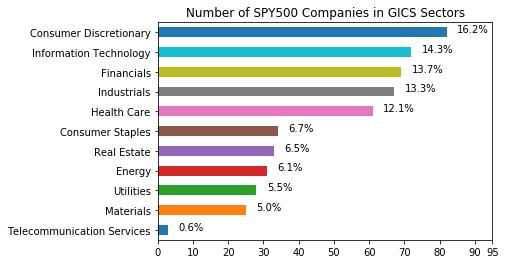
\includegraphics{images/traditional_sectors.jpeg}
    \caption{feature_selection:traditional_sectors}
    \label{fig:feature_selection:traditional_sectors}
\end{figure}

\end{document}